\section{Durchführung}
\label{sec:Durchführung}

Der Versuch wird \autoref{fig:aufbau} entsprechend aufgebaut.

\begin{figure}[H]
    \centering
    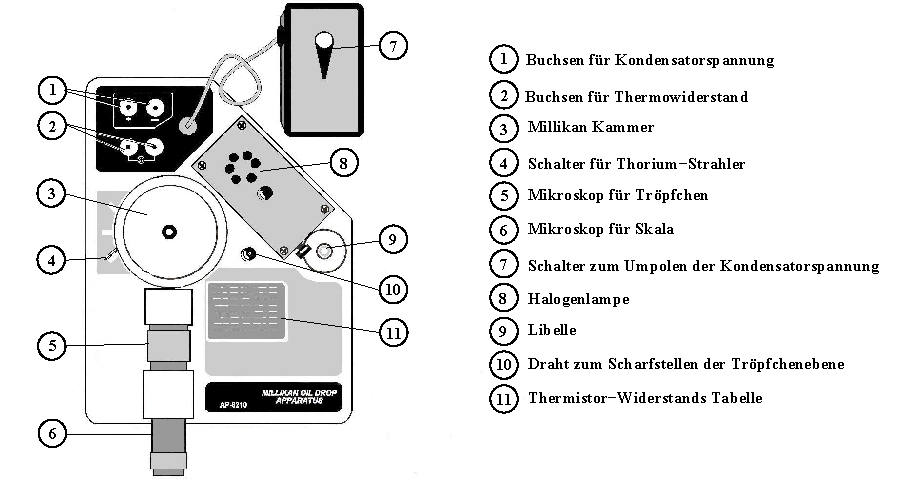
\includegraphics[]{figures/Aufbau.pdf}
    \caption{Beschriftete Abbildung des verwendeten Versuchsaufbaus \cite{v48}.}
    \label{fig:aufbau}
\end{figure}

Da die Probenkristalle hygroskopisch sind, wird mithilfe der Drehschieber-Vakuumpumpe im Rezipienten, der die Probe enthält, ein Vakuum von etwa $10^{-2} \,\si{\milli\bar}$ aufrechterhalten. 
Die Heizwicklung im Boden des Rezipienten ermöglicht ein Erwärmen der Probe.
Je nach Bedarf kann diese ebenfalls über Kühlfinger abgekühlt werden. Dazu wird das Dewargefäß mit flüssigem Stickstoff gefüllt und der Kühlfinger so weit aufgefahren, dass er hineintaucht. \\
Die Probentemperatur lässt sich über das im Boden des Rezipienten befindliche Thermoelement ablesen.
Über das angeschlossene Netzgerät kann der Heizstrom so angepasst werden, dass bei der Durchführung eine konstante Heizrate erreicht wird. \\
Eine genauere, schematische Darstellung des Rezipienten findet sich in \autoref{fig:rezipient}.

\begin{figure}[H]
    \centering
    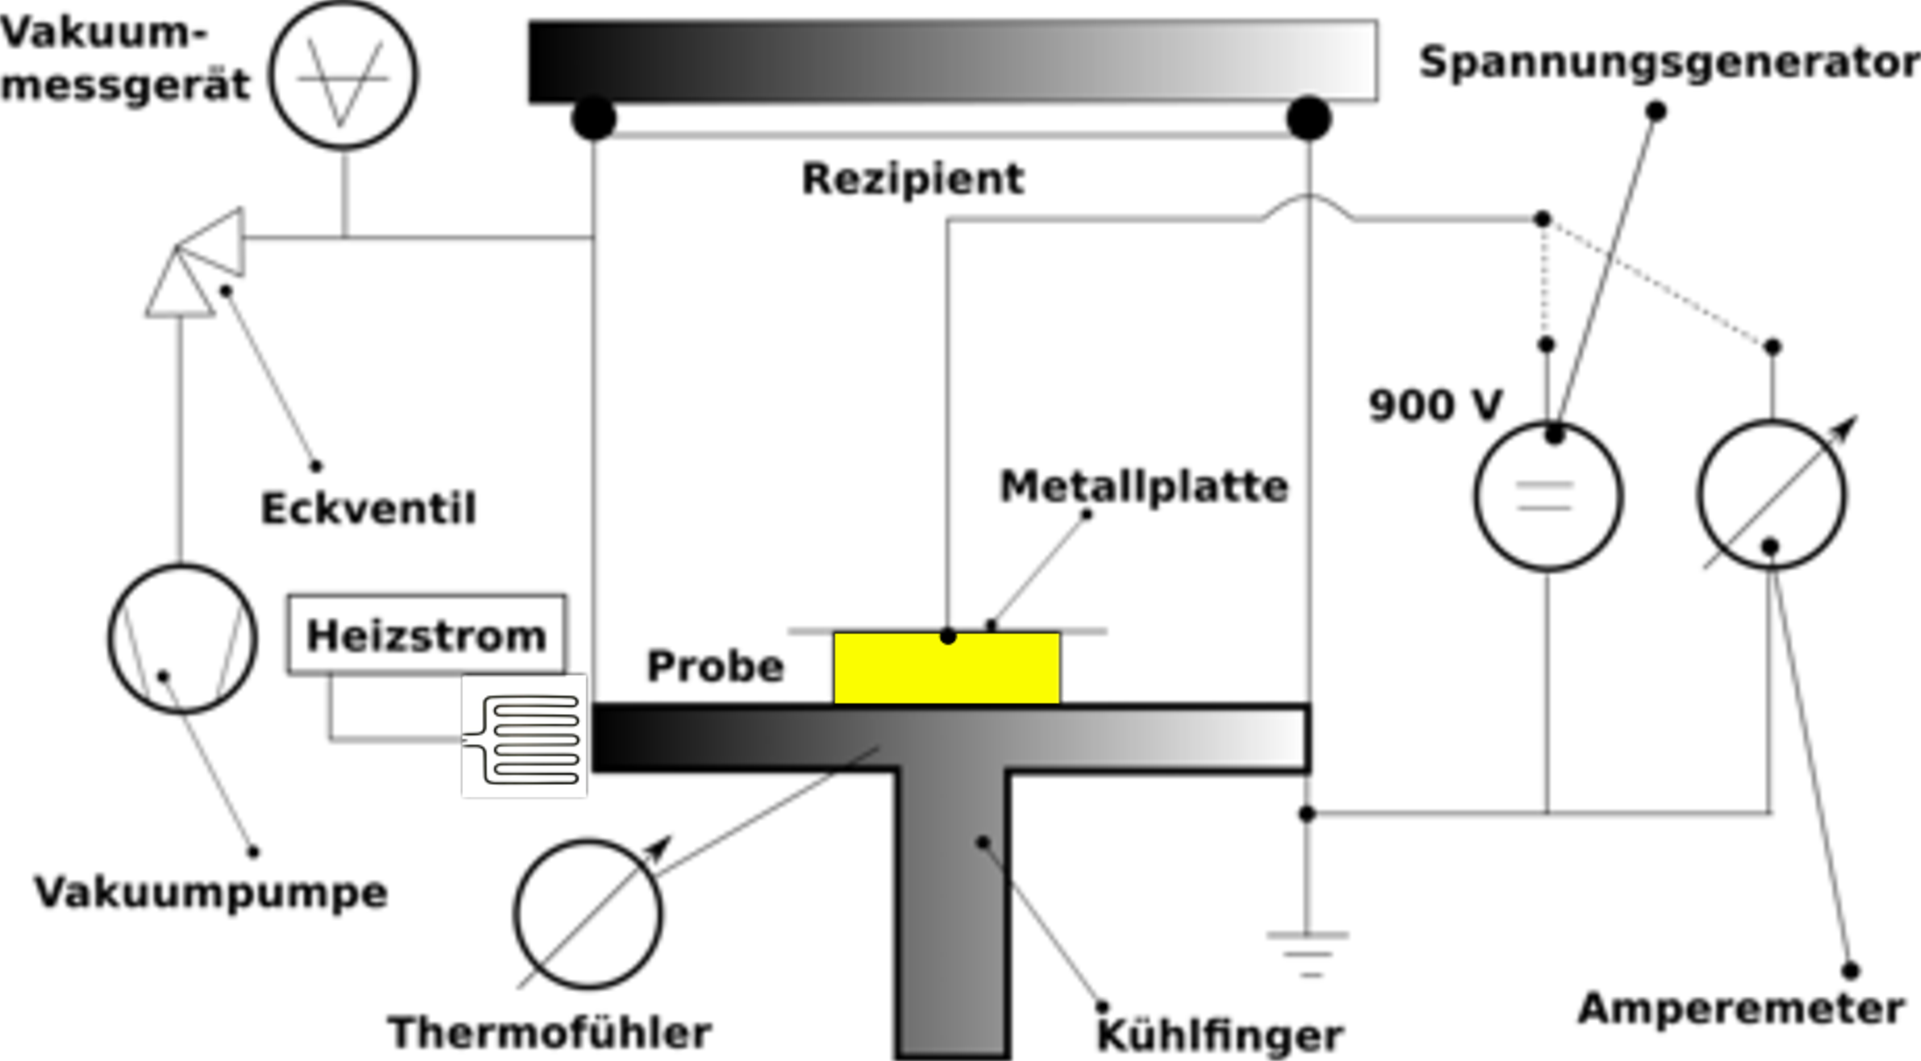
\includegraphics[]{figures/Rezipient.pdf}
    \caption{Schematische Darstellung des Rezipienten. In gelb ist die Probe dargestellt, die aufliegende Metallplatte ist dieser gegenüber ionisiert und der Rezipient geerdet \cite{v48}.}
    \label{fig:rezipient}
\end{figure}

Vor Beginn der eigentlichen Messreihe muss der Plattenkondensator durch Anlegen eines elektrischen Feldes mit einer Spannung von $950 \,\si{\volt}$ aufgeladen werden.
Dabei ist für die CsJ-Probe bei $295 \,\si{\kelvin}$ und die KBr-Probe bei $320 \,\si{\kelvin}$ eine Aufladezeit von $900 \,\si{\second}$ genügend.
Anschließend wird die Probe auf $210 \,\si{\kelvin}$ abgekühlt.
Sobald diese Temperatur erreicht ist, wird das E-Feld abgeschaltet und der Kondensator für $5 \si{\minute}$ kurzgeschlossen.
Nach Anschließen des Picoamperemeters sollte ein konstanter Stromwert zwischen $1-2 \,\si{\pico\ampere}$ erreicht werden, bevor mit der Messung begonnen wird.
Dann wird die Probe möglichst gleichmäßig auf etwa $330 \,\si{\kelvin}$ erwärmt und der Depolarisierungsstrom in Temperaturabhängigkeit aufgenommen.
Die Messung wird mit einer weiteren Heizrate wiederholt.